%Did it work properly? What kind of tests did you run to test your prototype? Could you provide some data that shows the performance of the prototype (speed, success rate, etc.)?

%Did it work probably?
\subsection{Implementation of project}
Our final end product ended up being very similar to our expected reference model. See figure \ref{fig:sbs} for a comparison of the reference model and the final implementation.
\begin{figure*}[h]
	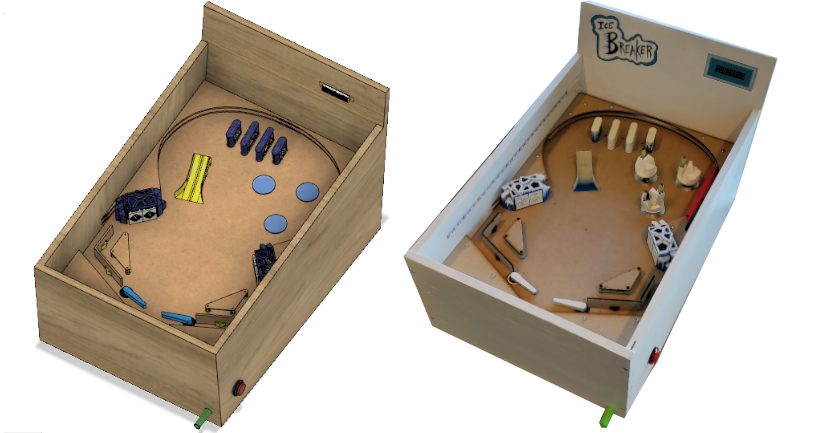
\includegraphics[width=\textwidth]{SideBySide}
	\caption{Side by side view of reference model (left) and image of final implementation (right). See Fusion 360 model named FinalAssembly for reference model.}
	\label{fig:sbs}
\end{figure*}
Individually we got every electronic mechanism/subcomponent working using an Arduino. When later combined, all the electronics software was loaded onto one Arduino Mega, which worked as expected. Please see the alongside submitted video for a presentation of the subcomponents working together on the assembled version.
\subsection{Shortcomings}
\subsubsection{Flippers}
During the final assembly, unfortunately the board used for distributing regulated power to the flippers broke. Although, as we proved during earlier tests, the layout worked as intended. For the final presentation, we did a workaround for showcasing the mechanism.
\subsubsection{Fall down mechanism}
Unfortunately the registration of a ball being lost, was de-scoped for the final presentation. We simply needed more time for tuning the sensor so that it worked reliably. Although the software for registration, counting and displaying lives are ready. 
\subsubsection{Ramp}
The ramp in the upper left corner of the playfield was originally intended to have rails for moving the ball across the playfield. Although due to time constrains, this was de-scoped. The final implementation although still has the ramp installed.
\subsection{The construction process}
\subsubsection{General}	
Since the project is made of many smaller subcomponents we had the chance to create these components independent of each other. This meant that we had the ability to test each component's mechanism, electronics and software separately before putting everything together. This way it was easier to test the project as a whole and to combine all the components to create the final prototype.\\
\subsubsection{Mechanism}
To make sure that the mechanism of a component was working, a model would first be created in Autodesk Fusion 360 and \textit{joined} together with other components if it interacted with them. Then one copy would be produced and tested. If the component worked, the rest of the components of the same type would be produced the same way, otherwise the 3D model would be configured to fit better and reproduced. This iterative process would continue until a successful component was created.\\
\subsubsection{Electronics}
Similar to the mechanisms, our electronic circuits were tested separately before expanded and soldered onto perf-board.
This was especially important, as we were dealing with multiple components that used either 5, 12 or 24 volts voltage. These were tested separately from the Arduino to avoid short circuits. We did this using buck boosts. 
\subsubsection{Software}
After we made sure the mechanisms and electronics worked for a component we added the software to it. Each component had their own Arduino-sketch class where all their own logic existed. Here we could test the code for each component and make sure that it worked as it should before declaring the component completely finished.
\\
To compensate for having all subcomponents logic on one Arduino, we had to rule out the often used "delay" method for waiting for a process. This event-driven process meant that no call was blocking. See appendix \ref{appendix:programming model} for further details about our programming model.
\\
Finally we combined all the Arduino-sketch classes into one main class.
